\documentclass[a4j]{jarticle}
    \usepackage[dvipdfmx]{graphicx}
    \usepackage[ top=25truemm,bottom=25truemm,left=25truemm,right=25truemm]
    {geometry}
    \usepackage{ascmac}
    \usepackage{array}
    \usepackage{here}
    \usepackage{here}
    \usepackage{listings, jlisting}
    \usepackage{url}
    \usepackage{multirow}
    \renewcommand{\lstlistingname}{リスト}
\lstset{language=c,
  basicstyle=\ttfamily\scriptsize,
  commentstyle=\textit,
  classoffset=1,
  keywordstyle=\bfseries,
  frame=tRBl,
  framesep=5pt,
  showstringspaces=false,
  numbers=left,
  stepnumber=1,
  numberstyle=\tiny,
  tabsize=4
}

\makeatletter
\def\@thesis{工学実験実習IV レポート}
\def\id#1{\def\@id{#1}}
\def\department#1{\def\@department{#1}}

\def\@maketitle{
\begin{center}
{\huge \@thesis \par} %修士論文と記載される部分
\vspace{10mm}
{\LARGE\bf \@title \par}% 論文のタイトル部分
\vspace{10mm}
{\Large \@date\par}	% 提出年月日部分
\vspace{20mm}
{\Large \@department \par}	% 所属部分
{\Large 学籍番号 \@id \par}	% 学籍番号部分
\vspace{10mm}
{\Large 氏名 \@author}% 氏名 
\end{center}
\par\vskip 1.5em
}

\title{SQL データベース}
\date{実験日1 2020年7月15日 1~2コマ目 \\ 実験日2 2020年7月21日 1~2コマ目 \\ 実験日3 2020年7月22日 1~2コマ目 \\ 実験日4 2020年7月29日 1~2コマ目 \\  実験日5 2020年8月05日 1~2コマ目 \\ 提出日 令和2年8月6日}
\department{組番号 408}
\id{17406}
\author{金澤雄大}

    \begin{document}
    \maketitle
    \thispagestyle{empty}
    \clearpage
    \addtocounter{page}{-1}
    \section{目的}
    多くのデータを扱いたいとき,ファイルにデータを保存し読み込むことで多くのデータを扱うことがある.しかしファイルを扱うと,複数人が同時に編集を
    扱うことや膨大な数のデータの検索や更新を行うことが難しい.そこでデータベースを利用する.このデータベースとやりとりする言語がSQL(Structured Query Language)
    である.本実験ではSQLの使い方を学習することを目的とする.また,データベースを効率よく格納し,拡張性を考慮したテーブルの定義として正規化がある.この正規化について
    理解し,実際に適用することを目的とする.さらに,国や地方公共団体が提供している実際のデータ(オープンデータ)を利用しデータベースを作成することを
    目的とする.また作成したデータベースの利用方法や有用性を考察することも目的とする.
    \section{理論・原理}
    本章では,データベースの概要,およびMySQLの基礎,および正規化とER図について述べる.
    \subsection{データベースの概要}
    「データベース」とはデータが保管されているものという意味である.コンピュータシステムにおける「データベース」はデータベースマネージメントシステム(DBMS)
    を指すことが多い.DBMSとはデータベースの管理,およびデータの抽出を代表とする読み書きを行うソフトウェアのことである.イメージとしては
    大量の本がある図書館がデータベースであり,本の検索や管理を行う図書館司書がDBMSである.DBMSには様々なものがあるが本実験ではMySQLを用いる.\\
     MySQLは命令(クリエという)を発行すると,DBMSを介してデータベースにアクセスし,クエリの要求に答える出力を行う.
    クエリは大別すると次のような種類のものがある.
    \begin{itemize}
      \item データの格納
      \item データの検索
      \item データの操作(追加,削除,更新)
      \item データの定義と関連付け
    \end{itemize}

    \subsection{MySQLの基礎}
    MySQLの基礎を説明するために用語の説明を行う.
    SQLにおいてデータを保存するための表を「テーブル」という.
    図\ref{db}はテーブルの例を示したものである.図\ref{db}ではテーブルAとテーブルBの2つがあることがわかる.図\ref{db}に示した,データの項目をカラムという.
    図\ref{db}のテーブルAにおけるカラムは,ID,学籍番号,名前の3つである.また,1行分のデータをレコードという.図\ref{db}のテーブルAおよびテーブルBは2つのレコードがあることが読み取れる.
    複数のテーブルを集めたものをデータベースと呼ぶ.図\ref{db}のデータベースDは,テーブルAとテーブルBの2つのテーブルをもっている
    データベースであることがわかる.
    \begin{figure}[H]
      \centering
      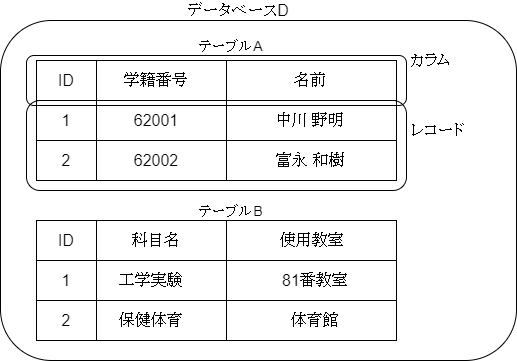
\includegraphics[scale=0.5]{db.png}
      \caption{データベースとテーブル}
       \label{db}
      \end{figure}

    本実験ではデータベースにおけるデータの格納方法として「リレーショナルデータベース」を用いる.リレーショナルデータベースとは
    テーブルにカラムが設定され,レコードが記録されたテーブルが相互に関係をとることで,要求にあったデータを抽出することができるような仕組みを
    持つデータベースのことである.\\
     またSQLはC言語やJavaのように格納するデータの型が存在する.データ型は数値型,日付型,文字列型の3つがある.
    表\ref{numerical},および表\ref{date},および表\ref{string}に各型の代表的なデータ型を示す.また,表\ref{numerical}
    に示した数値型の他に,浮動小数点を扱うFLOAT型およびDOUBLE型が存在する.
    
\begin{table}[H]
	\caption{数値型の代表例}
	\label{numerical}
	\begin{center}
		\begin{tabular}{l|r|r|r}\hline
      \multirow{2}{*}{型} & \multirow{2}{*}{ストレージ(バイト)} & 最小値 & 最大値 \\ \cline{3-4}
       & & 符号付き/符号なし &  符号付き/符号なし \\ \hline \hline
      \multirow{2}{*}{TINYINT} & \multirow{2}{*}{1} & -128 & 127 \\ \cline{3-4}
       & & 0 &  255 \\ \hline
       \multirow{2}{*}{SMALLINT} & \multirow{2}{*}{2} & -32768 & 32767 \\ \cline{3-4}
       & & 0 &  65535 \\ \hline
       \multirow{2}{*}{MEDIUMINT} & \multirow{2}{*}{3} & -8388608  & 8388607 \\ \cline{3-4}
       & & 0 & 16777215 \\ \hline
       \multirow{2}{*}{INT} & \multirow{2}{*}{4} & -2147483648 & 2147483647 \\ \cline{3-4}
       & & 0 & 4294967295 \\ \hline
       \multirow{2}{*}{BIGINT} & \multirow{2}{*}{8} & -9223372036854775808 & 9223372036854775807 \\ \cline{3-4}
       & & 0 &  18446744073709551615 \\ \hline
 		\end{tabular}
	\end{center}
  \end{table}


  \begin{table}[H]
    \caption{日付型の代表例}
    \label{date}
    \begin{center}
      \begin{tabular}{l|l|c}\hline
        型 & 内容 & 型/範囲 \\ \hline \hline
        DATE & 日付部分(時間部分は含まない) & \begin{tabular}{c} 'YYYY-MM-DD' \\ '1000-01-01'~'9999-12-31' \end{tabular} \\ \hline
        DATETIME & 日付と時間の両方 & \begin{tabular}{c}'YYYY-MM-DD HH:MM:SS' \\ '1000-01-01 00:00:00'~'9999-12-31 23:59:59' \end{tabular} \\ \hline
        TIMESTAMP & 日付と時間の両方 & \begin{tabular}{c} '1970-01-01 00:00:01' UTC \\ ~'2038-01-19 03:14:07' UTC \end{tabular} \\ \hline
       \end{tabular}
    \end{center}
    \end{table}
  
    \begin{table}[H]
      \caption{文字列型の代表例}
      \label{string}
      \begin{center}
        \begin{tabular}{l|l|c}\hline
          型 & 内容 & 範囲 \\ \hline \hline
          CHAR & 固定文字列 & 0から255までの任意の値 \\ \hline
          VARCHAR & 可変長文字列 & 0から65535までの値 \\ \hline
         \end{tabular}
      \end{center}
      \end{table}

    データベースの構築を行うときに用いる用語について説明する.図\ref{db}に示したように,各表のテーブル名およびカラム名が登場する項目そのままの
    名前で表されているモデルを論理モデルという.実際にデータベースを構築することを考えると,テーブル名およびカラム名が日本語であると文字コードの
    トラブルが起きる可能性がある.そこでテーブル名およびカラム名を英数字のみの構成にする.このようなモデルを物理モデルと呼ぶ.
    例として,図\ref{db}のデータベースでは,「名前」を「name」,「科目名」を「subject」に置き換える.
    \subsection{正規化とER図}
      正規化とはデータベースにデータを効率よく格納し,拡張性を考慮した,データベースの定義方法のことである.
      本実験では第一正規化,第二正規化,第三正規化と呼ばれる3つの正規化を行う.\\
       まず,第一正規化について説明する.表\ref{before}に第一正規化を行う前のデータを示す.
      \begin{table}[H]
        \caption{正規化する前のデータ}
        \label{before}
        \begin{center}
          \begin{tabular}{c|c|c|c|l|c|r}\hline
            学籍番号 & 学年 & 名前 & 学科 & 科目 & 担当者 & 点数  \\ \hline \hline
            \multirow{2}{*}{22421} & \multirow{2}{*}{4} &\multirow{2}{*}{田中 次郎} & \multirow{2}{*}{電子情報工学科} & データベース & 中村 剛 & 90  \\ \cline{5-7}
            &  &  &  & 電子回路 & 和田 知子 & 100 \\ \hline
            \multirow{2}{*}{22310} & \multirow{2}{*}{4} &\multirow{2}{*}{中村 花子} & \multirow{2}{*}{電子制御工学科} & 制御工学 & 江田 純也 & 87  \\ \cline{5-7}
            &  &  &  & 材料工学 & 藤枝 明彦 & 68 \\ \hline
            22315 & 4 & 成田 翼 & 電子制御工学科 & 材料工学 & 藤枝 明彦 & 89  \\ \hline
            21504 & 3 & 木村 剛 & 環境都市工学科 & 都市計画 & 内川 早苗 & 89  \\ \hline
           \end{tabular}
        \end{center}
        \end{table}

        第一正規化はレコードをまたいで定義される値がないように1レコードごとに分離する.表\ref{one}に
        表\ref{before}を第一正規化したテーブルを示す.表\ref{before}においてレコードをまたいで
        定義されている学籍番号,学年,名前,学科の4つのカラムが,レコードをまたがないように分離されている
        ことが読み取れる.
        \begin{table}[H]
          \caption{第一正規化したデータ}
          \label{one}
          \begin{center}
            \begin{tabular}{c|c|c|c|l|c|r}\hline
              学籍番号 & 学年 & 名前 & 学科 & 科目 & 担当者 & 点数  \\ \hline \hline
              22421 & 4 & 田中 次郎 & 電子情報工学科 & データベース & 中村 剛 & 90  \\ \hline
              22421 & 4 & 田中 次郎 & 電子情報工学科 & 電子回路 & 和田 知子 & 100 \\ \hline
              22310 & 4 & 中村 花子 & 電子制御工学科 & 制御工学 & 江田 純也 & 87  \\ \hline
              22310 & 4 & 中村 花子 & 電子制御工学科 & 材料工学 & 藤枝 明彦 & 68 \\ \hline
              22315 & 4 & 成田 翼 & 電子制御工学科 & 材料工学 & 藤枝 明彦 & 89  \\ \hline
              21504 & 3 & 木村 剛 & 環境都市工学科 & 都市計画 & 内川 早苗 & 89  \\ \hline
             \end{tabular}
          \end{center}
          \end{table}

        第一正規化したデータをもとに第二正規化を行う.第二正規化は主となるカラムとそれに従属するカラムを分離する.
        ここで,主となるカラムを主キー(PRIMARY KEY)という.主キーは重複することを許さない.
        例えば,学籍番号を主として,学年,名前,学科の3つが定まる.また,科目を主として担当者が決まる.さらに,学籍番号を主と
        科目に応じて科目の点数が決まる.すなわち,学生に関するテーブル,科目に関するテーブル,点数に関するテーブルの3つができあがる.
        表\ref{student2},および表\ref{subject2}および,表\ref{score2}にこの3つのテーブルを示す.
        \begin{table}[H]
          \caption{学生に関するテーブル(第二正規化)}
          \label{student2}
          \begin{center}
            \begin{tabular}{c|c|c|c}\hline
              学籍番号 & 学年 & 名前 & 学科 \\ \hline \hline
              22421 & 4 & 田中 次郎 & 電子情報工学科 \\ \hline
              22310 & 4 & 中村 花子 & 電子制御工学科 \\ \hline
              22315 & 4 & 成田 翼 & 電子制御工学科 \\ \hline
              21504 & 3 & 木村 剛 & 環境都市工学科 \\ \hline
             \end{tabular}
          \end{center}
          \end{table}

        \begin{table}[H]
          \begin{center}
            \begin{tabular}{c}

              \begin{minipage}{0.5\hsize}
          \caption{科目に関するテーブル(第二正規化)}
            \label{subject2}
            \begin{center}
              \begin{tabular}{c|c}\hline
                科目名& 担当者 \\ \hline \hline
                データベース & 中村 剛 \\ \hline 
                電子回路 & 和田 知子 \\ \hline
                制御工学 & 江田 純也 \\ \hline
                材料力学 & 藤枝 明彦 \\ \hline
                都市計画 & 内川 早苗 \\ \hline
             \end{tabular}
          \end{center}
        \end{minipage}

        \begin{minipage}{0.5\hsize}
          \caption{点数に関するテーブル(第二正規化)}
          \label{score2}
          \begin{center}
            \begin{tabular}{c|c|c}\hline
              学籍番号 & 科目名 & 点数 \\ \hline \hline
              22421 & データベース & 90 \\ \hline
              22421 & 電子回路 & 100 \\ \hline
              22310 & 制御工学 & 87 \\ \hline
              22310 & 材料力学 & 68 \\ \hline
              22315 & 材料力学 & 89 \\ \hline
              21504 & 都市計画 & 89 \\ \hline
               \end{tabular}
            \end{center}
          \end{minipage}
        \end{tabular}
      \end{center}
            \end{table}


          第三正規化は,第二正規化されたテーブルで従属関係を分離できていない部分を分離する.
          また,性別や学科のように選択肢から選ぶ項目を別のテーブルに抜き出す(LGBTの観点から性別を分けようとすると
          非常に複雑になってしまうためここでは男/女とする).表\ref{student3}~表\ref{score3}に第二正規化されたテーブルを第三正規化した
          テーブルを示す.第二正規化からの変更点は,表\ref{gakka3}に示すように学科に関するテーブルを設けて,学生に関するテーブル(表\ref{student3})からは学科IDで取り扱う.
          ただしここでの学科は本校の学科を暗に仮定している.こうすることで人間による表記ゆれ(例えば「電子 情報工学科」,「電子情報 工学科」)を防ぐことができる.
          また,科目に関するテーブル(表\ref{subject3})を設け点数に関するテーブル(表\ref{score3})からは科目を科目IDで扱う.
          \begin{table}[H]
            \begin{center}
              \begin{tabular}{c}

                \begin{minipage}{0.5\hsize}
            \caption{学生に関するテーブル(第三正規化)}
            \label{student3}
            \begin{center}
              \begin{tabular}{c|c|c|c}\hline
                学籍番号 & 学年 & 名前 & 学科 \\ \hline \hline
                22421 & 4 & 田中 次郎 & 4 \\ \hline
                22310 & 4 & 中村 花子 & 3 \\ \hline
                22315 & 4 & 成田 翼 & 3 \\ \hline
                21504 & 3 & 木村 剛 & 5 \\ \hline
               \end{tabular}
            \end{center}
          \end{minipage}

          \begin{minipage}{0.5\hsize}
            \caption{学科に関するテーブル(第三正規化)}
            \label{gakka3}
            \begin{center}
              \begin{tabular}{c|c}\hline
                学科ID & 学科名 \\ \hline \hline
                1 & 機械工学科 \\ \hline
                2 & 電気電子工学科 \\ \hline
                3 & 電子制御工学科 \\ \hline
                4 & 電子情報工学科 \\ \hline
                5 & 環境都市工学科 \\ \hline
               \end{tabular}
            \end{center}
          \end{minipage}
        \end{tabular}
      \end{center}
            \end{table}



            \begin{table}[H]
              \begin{center}
                \begin{tabular}{c}

              \begin{minipage}{0.5\hsize}
              \caption{科目に関するテーブル(第三正規化)}
              \label{subject3}
              \begin{center}
                \begin{tabular}{c|c|c}\hline
                  科目ID & 科目名 & 担当者 \\ \hline \hline
                  10001 & データベース & 中村 剛 \\ \hline 
                  10002 & 電子回路 & 和田 知子 \\ \hline
                  10003 & 制御工学 & 江田 純也 \\ \hline
                  10004 & 材料力学 & 藤枝 明彦 \\ \hline
                  10005 & 都市計画 & 内川 早苗 \\ \hline
                 \end{tabular}
              \end{center}
            \end{minipage}

            \begin{minipage}{0.5\hsize}
                \caption{点数に関するテーブル(第三正規化)}
                \label{score3}
                \begin{center}
                  \begin{tabular}{c|c|c}\hline
                    学籍番号 & 科目名 & 点数 \\ \hline \hline
                    22421 & 10001 & 90 \\ \hline
                    22421 & 10002 & 100 \\ \hline
                    22310 & 10003 & 87 \\ \hline
                    22310 & 10004 & 68 \\ \hline
                    22315 & 10004 & 89 \\ \hline
                    21504 & 10005 & 89 \\ \hline
                   \end{tabular}
                \end{center}
              \end{minipage}
            \end{tabular}
          \end{center}
                \end{table}

    第一正規化から第三正規化を行い,4つのテーブルができた.4つ程度のテーブルで構成されるデータベースであれば,テーブルの関係が
    わかるかもしれないが,実際に扱うテーブルはそれよりも多いと考えられる.テーブルが増えると,テーブルの関係がより複雑になり,
    簡単に把握することが難しくなる.そこで,ER図というものを用いてテーブル同士の関係を図で表すことでテーブルの関係を
    明快にすることができる.図\ref{ronri}および図\ref{buturi}に第三正規化した4つのテーブルをER図にしたものを示す.
    図\ref{ronri}は論理モデルにおけるER図,図\ref{buturi}は物理モデルにおけるER図を示している.ER図の見方は,
    囲いの外側に書かれている文字がテーブル名である.囲いの上から一段目に書かれているカラムが主キー,二段目に書かれているカラムが
    主キーに従属するキーである.また(FK)とはFOREIGN KEY(外部キー)のことで入力を別のテーブルの特定のカラムのデータに
    制限する.またテーブル間の線はテーブルに依存関係があるか否かを示している.

    \begin{figure}[H]
      \centering
      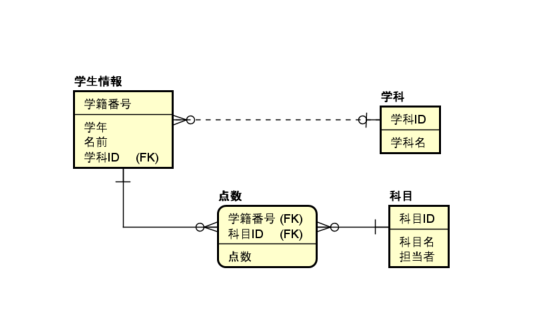
\includegraphics[scale=1.4]{ronti.png}
      \caption{ER図の例(論理モデル)}
       \label{ronri}
      \end{figure}

      \begin{figure}[H]
        \centering
        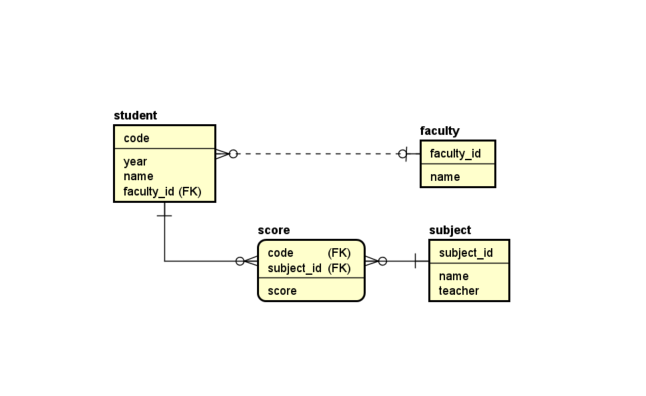
\includegraphics[scale=1.4]{buturi.png}
        \caption{ER図の例(物理モデル)}
         \label{buturi}
        \end{figure}

        astahでER図を作成する場合,作成したER図からテーブルを作成するクエリを発行することができる.
        本実験ではこの機能を利用してMySQLのテーブル定義を行う.

    \section{実験方法}
    本章では実験環境,および実験の手順および内容について述べる.本実験ではER図の作成にastahを用いる.
    また,MySQLのソースコードにおいて,命令は大文字で表記するものとする.
    \subsection{実験環境}
    \begin{table}[H]
      \caption{実験環境}
      実験環境を表\ref{kankyou}に示す.
      \label{kankyou}
      \begin{center}
          \begin{tabular}{l|c}\hline
            CPU & Intel Core i7-6500 2.50Ghz \\ 
            メモリ & 16.0GB DDR3 \\
            OS & Windows 10 Home \\
            MySQL & version8.0.19 Community Server - GPL \\ 
            astah professional  & version 8.2.0/b743f7 \\
            文字コード & UTF-8 \\ \hline
          \end{tabular}
      \end{center}
      \end{table}

    \subsection{実験の手順および内容}
    実験として授業中に与えられた課題を4つ行う.本節では4つの課題の内容について述べる.
    \subsubsection{課題1}
      表\ref{kadai1}に示すテーブルについて第一正規化~第三正規化を行いER図を作成する.ただし条件は次の通りである.
      \begin{itemize}
        \item 担当コードおよび学籍番号は1人につき1つ付与されていて,ユニークな値である.
        \item 同じ科目名の科目は複数存在しない.
        \item 1つの科目の担当者は必ず1名である.
        \item 成績の入力日は入力した日付とする.
        \item 学科および校舎は本校の場合を仮定する\cite{NNCT}.学科の一覧は表\ref{gakka3}に示したものを利用する.校舎の一覧は表\ref{kosha}に示す.
        \item 性別は男/女のどちらかとする.
        \item 判定は表\ref{hantei}に示す方法で方法で決定する.
      \end{itemize}
      
      \begin{table}[H]
        \caption{学生成績表}
        \label{kadai1}
        \begin{center}
          \scalebox{0.7}[0.9]{
          \begin{tabular}{c|c|c|c|c|c|c|c|c|c|c|c}\hline
            学籍番号 & 学生名 & 年齢 &性別 & 学科 & 校舎 & 科目名 & 点数 & 判定 & 教員コード & 教員名 & 入力日 \\ \hline \hline
            \multirow{3}{*}{26401} & \multirow{3}{*}{山川 一郎} & \multirow{3}{*}{18} & \multirow{3}{*}{男} & \multirow{3}{*}{電子情報工学科} & \multirow{3}{*}{電子情報工学科棟}
            & 国語II & 65 & 可 & G002 & 長松次郎 & 2018-06-10 \\ \cline{7-12}
             & & & & & & 物理I & 42 & 不可 & G001 & 長松 遥 & 2018-06-11 \\ \cline{7-12}
             & & & & & & 現代社会 & 79 & 良 & G005 & 高田 真由 & 2018-06-14 \\ \hline
             \multirow{3}{*}{26205} & \multirow{3}{*}{谷川 太郎} & \multirow{3}{*}{19} & \multirow{3}{*}{男} & \multirow{3}{*}{電気電子工学科} & \multirow{3}{*}{電気電子・機械工学科棟}
             & 物理I & 76 & 良 & G001 & 長松 遥 & 2018-06-11 \\ \cline{7-12}
              & & & & & & 電気工学 & 66 & 可 & E012 & 三浦 裕 & 2018-06-12 \\ \cline{7-12}
              & & & & & & 信号処理 & 90 & 優 & E012 & 三浦 裕 & 2018-06-12 \\ \hline
            \multirow{3}{*}{26132} & \multirow{3}{*}{海土 花子} & \multirow{3}{*}{20} & \multirow{3}{*}{女} & \multirow{3}{*}{機械工学科} & \multirow{3}{*}{電気電子・機械工学科棟}
             & 物理I & 87 & 優 & G001 & 長松 遥 & 2018-06-10 \\ \cline{7-12}
              & & & & & & 機械工学 & 78 & 良 & M301 & 上条 雄三 & 2018-06-11 \\ \cline{7-12}
              & & & & & & 計測工学 & 100 & 優 & M533 & 西岡 剛 & 2018-06-12 \\ \hline  
           \end{tabular}
          }
        \end{center}
        \end{table}

        \begin{table}[H]
          \begin{center}
            \begin{tabular}{c}
             
              \begin{minipage}{0.5\hsize}
          \caption{校舎の一覧}
          \label{kosha}
          \begin{center}
            \begin{tabular}{c|c}\hline
              校舎ID & 校舎名 \\ \hline \hline
              1 & 管理・一般校舎 \\ \hline 
              2 & 電子制御工学科棟 \\ \hline 
              3 & 電気電子・機械工学科棟 \\ \hline 
              4 & 電子情報工学科棟 \\ \hline 
              5 & 環境都市工学科棟 \\ \hline 
              6 & 情報教育センター \\ \hline 
              7 & 図書館センター \\ \hline 
              8 & 体育館 \\ \hline 
             \end{tabular}
          \end{center}
        \end{minipage}

        \begin{minipage}{0.5\hsize}
            \caption{成績の判定方法}
            \label{hantei}
            \begin{center}
              \begin{tabular}{c|c|c}\hline
                判定 & 最小値 & 最大値 \\ \hline \hline
                不可 & 0 & 59 \\ \hline
                可 & 60 & 69 \\ \hline
                良 & 70 & 79\\ \hline
                優 & 80 & 100\\ \hline
               \end{tabular}
            \end{center}
          \end{minipage}
        \end{tabular}
      \end{center}
            \end{table}

    \subsubsection{課題2}
    課題1で正規化したテーブルおよびER図を用いて,MySQLにデータベースおよびテーブルを定義する.また定義したテーブルに
    レコードを格納するクエリを発行し,各テーブルに登録したデータの内容を表示する.
    カラムの物理名,物理,型,必須/非必須(データがNULLであることを許すか)は表\ref{joken}に従うとする.

    \begin{table}[H]
      \caption{カラムの設定}
      \label{joken}
      \begin{center}
        \begin{tabular}{l|l|l|l|l}\hline
          項目 & カラム(論理名) & カラム(物理名) & 型 & 必須/非必須 \\ \hline \hline
          学籍番号 & 学籍番号 & code & CHAR(5) & 必須 \\ \hline
          学生名 & 名前 & name & VARCHAR(40) & 必須 \\ \hline
          年齢 & 年齢 & age & INT & 非必須 \\ \hline
          性別 & 性別 & gender & CHAR(4) & 非必須 \\ \hline
          学科 & 学科 & faculty & VARCHAR(40) & 必須 \\ \hline
          校舎 & 校舎 & place & VARCHAR(40) & 必須 \\ \hline
          科目名 & 科目名 & subject & CVARHAR(40) & 必須 \\ \hline
          教員コード & 教員コード & teacher\_id & CHAR(4) & 必須 \\ \hline
          教員名 & 名前 & name & VARCHAR(40) & 必須 \\ \hline
          点数 & 点数 & score & INT & 必須 \\ \hline
          判定 & 判定 & result & VARCHAR(6) & 必須 \\ \hline
          入力日 & 入力日 & date & DATE & 必須 \\ \hline
        \end{tabular}
      \end{center}
      \end{table}

    \subsubsection{課題3}
    課題2で登録したデータに対し,次に示す5つのクエリを発行し,実行する.
    \begin{enumerate}
      \item 第一正規化したときの表を表示するクエリ.
      \item いずれかの科目の判定が「優」である学生の学籍番号,氏名,学科を問い合わせるクエリ.
      \item 担当者が「高田」,または「三浦」である科目を履修している学生について,学生名,科目名,点数を問い合わせるクエリ.
      \item 科目名に「学」が含まれる科目について,履修している学生名,科目名,点数を問い合わせるクエリ.
      \item 担当が「三浦」の科目の低近点を問い合わせるクエリ.
    \end{enumerate}
    \subsubsection{課題4}
    オープンデータについて,課題1から3と同様の処理を行う.すなわちオープンデータについて第三正規化までを行い,ER図を作成する.
    さらにデータベースおよびテーブル定義を行うクエリを発行し,実行する.最後に課題3のようにデータを問い合わせる
    クエリを発行し,実行する.
    \section{課題1}
    本章では3つの正規化の過程および結果について述べる.
    \subsection{第一正規化の結果}
    表\ref{kadai1}に示すデータを第一正規化する.第一正規化とはレコードをまたいで定義されるカラムを
    レコードをまたがないように分離する操作であった.表\ref{kadai1}のデータでは,学生名,年齢,性別,学科,校舎の
    5つのカラムがレコードをまたいでいることがわかる.これより,これらのカラムについて,レコードをまたがないように変更する.
    表\ref{one1}に表\ref{kadai1}のデータを正規化したデータを示す.表\ref{one1}ではレコードをまたいで定義されるカラムが
    ないことがわかる.

    \begin{table}[H]
      \caption{第一正規化の結果}
      \label{one1}
      \begin{center}
        \scalebox{0.7}[0.9]{
        \begin{tabular}{c|c|c|c|c|c|c|c|c|c|c|c}\hline
          学籍番号 & 学生名 & 年齢 & 性別 & 学科 & 校舎 & 科目名 & 点数 & 判定 & 教員コード & 教員名 & 入力日 \\ \hline \hline
26401 & 山川一郎 & 18 & 男 & 電子情報工学科 & 電子情報工学科棟 & 国語II & 65 & 可 & G002 & 長松次郎 & 2018/6/10 \\ \hline
26401 & 山川一郎 & 18 & 男 & 電子情報工学科 & 電子情報工学科棟 & 物理I & 42 & 不可 & G001 & 長松遥 & 2018/6/11 \\ \hline
26401 & 山川一郎 & 18 & 男 & 電子情報工学科 & 電子情報工学科棟 & 現代社会 & 79 & 良 & G005 & 高田真由 & 2018/6/14 \\ \hline
26205 & 谷泉太郎 & 19 & 男 & 電気電子工学科 & 電気電子・機械工学科棟 & 物理I & 76 & 良 & G001 & 長松遥 & 2018/6/11 \\ \hline
26205 & 谷泉太郎 & 19 & 男 & 電気電子工学科 & 電気電子・機械工学科棟 & 電気工学 & 66 & 可 & E012 & 三浦裕 & 2018/6/12 \\ \hline
26205 & 谷泉太郎 & 19 & 男 & 電気電子工学科 & 電気電子・機械工学科棟 & 信号処理 & 90 & 優 & E012 & 三浦裕 & 2018/6/12 \\ \hline
26132 & 海土花子 & 20 & 女 & 機械工学科 & 電気電子・機械工学科棟 & 物理I & 87 & 優 & G001 & 長松遥 & 2018/6/10 \\ \hline
26132 & 海土花子 & 20 & 女 & 機械工学科 & 電気電子・機械工学科棟 & 機械力学 & 78 & 良 & M301 & 上条雄三 & 2018/6/11 \\ \hline
26132 & 海土花子 & 20 & 女 & 機械工学科 & 電気電子・機械工学科棟 & 計測工学 & 100 & 優 & M553 & 西岡剛 & 2018/6/12  \\ \hline
        \end{tabular}
        }
      \end{center}
      \end{table}

    \subsection{第二正規化の結果}
    表\ref{one1}のデータを第二正規化する.第二正規化とは主となるカラムと,それに従属するカラムにデータを分離する
    ことであった.表\ref{one1}を見ると,学籍番号を主として,学生名,年齢,性別,学科,校舎の5つが定まることがわかる.
    また科目名を主として,教員コードと教員名が定まる.同様に,学籍番号と科目名の2つを主として,点数,判定,入力日の3つが定まる.
    すなわち,第二正規化によって3つのテーブルが出来上がる.説明のために,それぞれのテーブルを学生テーブル,科目テーブル,成績
    テーブルと呼ぶことにする.表\ref{one2A}~表\ref{one2C}に第二正規化によってできる3つのテーブルを示す.
    \begin{table}[H]
      \caption{学生テーブル(第二正規化)}
      \label{one2A}
      \begin{center}
        \begin{tabular}{c|c|c|c|c|c}\hline
          学籍番号 & 学生名 & 年齢 & 性別 & 学科 & 校舎 \\ \hline \hline
          26401 & 山川一郎 & 18 & 男 & 電子情報工学科 & 電子情報工学科棟 \\ \hline
          26205 & 谷泉太郎 & 19 & 男 & 電気電子工学科 & 電気電子・機械工学科棟 \\ \hline
          26132 & 海土花子 & 20 & 女 & 機械工学科 & 電気電子・機械工学科棟 \\ \hline
        \end{tabular}
      \end{center}
      \end{table}

    \begin{table}[H]
      \begin{center}
        \begin{tabular}{c}

          \begin{minipage}{0.5\hsize}
      \caption{科目テーブル(第二正規化)}
      \label{one2B}
      \begin{center}
        \begin{tabular}{c|c|c}\hline
          科目名 & 教員コード & 教員名 \\ \hline \hline
          国語II & G002 & 長松次郎 \\ \hline
          物理I & G001 & 長松遥 \\ \hline
          現代社会 & G005 & 高田真由 \\ \hline
          電気工学 & E012 & 三浦裕 \\ \hline
          信号処理 & E012 & 三浦裕 \\ \hline
          機械力学 & M301 & 上条雄三 \\ \hline
          計測工学 & M553 & 西岡剛 \\ \hline
        \end{tabular}
      \end{center}
    \end{minipage}

    \begin{minipage}{0.5\hsize}
        \caption{成績テーブル(第二正規化)}
        \label{one2C}
        \begin{center}
          \begin{tabular}{c|c|c|c|c}\hline
            学籍番号 & 科目名 & 点数 & 判定 & 入力日 \\ \hline \hline
26401 & 国語II & 65 & 可 & 2018/6/10 \\ \hline
26401 & 物理I & 42 & 不可 & 2018/6/11 \\ \hline
26401 & 現代社会 & 79 & 良 & 2018/6/14 \\ \hline
26205 & 物理I & 76 & 良 & 2018/6/11 \\ \hline
26205 & 電気工学 & 66 & 可 & 2018/6/12 \\ \hline
26205 & 信号処理 & 90 & 優 & 2018/6/12 \\ \hline
26132 & 物理I & 87 & 優 & 2018/6/10 \\ \hline
26132 & 機械力学 & 78 & 良 & 2018/6/11 \\ \hline
26132 & 計測工学 & 100 & 優 & 2018/6/12 \\ \hline
          \end{tabular}
        \end{center}
      \end{minipage}
    \end{tabular}
  \end{center}
        \end{table}
    

    \subsection{第三正規化の結果}
    第二正規化した結果を元に第三正規化を行う.第三正規化とは,第二正規化で分離できていない従属関係を
    分離し,選択肢から選ぶ項目を抜き出す操作であった.学生テーブル(表\ref{one2A})では,性別と学科は
    選択肢から選ぶ項目であるから抜き出してよいと考える.また校舎は学科によって定まるものであるため,
    校舎は学科から参照する形に変更する.科目テーブル(表\ref{one2B})では,教員名は教員コードで一意に定まる
    ものであるから,教員名を教員コードから参照する形に変更する.成績テーブル(表\ref{one2C})では,判定は点数に
    よって定まるから,判定を成績テーブルから分離する.点数から判定を決定する方法は上限,下限を用いてSQLのクエリ
    から計算を行うようにする.これより,第三正規化によって8つのテーブルができることがわかる.
    表\ref{one3A}~\ref{one3H}に8つのテーブルを示す.

    \begin{table}[H]
      \begin{center}
        \begin{tabular}{c}

          \begin{minipage}{0.5\hsize}
      \caption{学生テーブル(第三正規化)}
      \label{one3A}
      \begin{center}
        \begin{tabular}{c|c|c|c|c}\hline
          学籍番号 & 学生名 & 年齢 & 性別 & 学科 \\ \hline \hline
          26401 & 山川一郎 & 18 & 0 & 4 \\ \hline 
          26205 & 谷泉太郎 & 19 & 0 & 2 \\ \hline 
          26132 & 海土花子 & 20 & 1 & 1 \\ \hline 
        \end{tabular}
      \end{center}
    \end{minipage}

    \begin{minipage}{0.5\hsize}
        \caption{性別テーブル(第三正規化)}
        \label{one3B}
        \begin{center}
          \begin{tabular}{c|c}\hline
            性別ID & カテゴリ  \\ \hline \hline
            1 & 男  \\ \hline
            2 & 女  \\ \hline
          \end{tabular}
        \end{center}
      \end{minipage}
    \end{tabular}
  \end{center}
        \end{table}

        \begin{table}[H]
          \begin{center}
            \begin{tabular}{c}

              \begin{minipage}{0.5\hsize}
          \caption{学科テーブル(第三正規化)}
          \label{one3C}
          \begin{center}
            \begin{tabular}{c|c|c}\hline
              学科ID & 学科 & 校舎ID  \\ \hline \hline
              1 & 機械工学科 & 3  \\ \hline
              2 & 電気電子工学科 & 3  \\ \hline
              3 & 電子制御工学科 & 2  \\ \hline
              4 & 電子情報工学科 & 4  \\ \hline
              5 & 環境都市工学科 & 5  \\ \hline
            \end{tabular}
          \end{center}
        \end{minipage}

        \begin{minipage}{0.5\hsize}
            \caption{校舎テーブル(第三正規化)}
            \label{one3D}
            \begin{center}
              \begin{tabular}{c|c}\hline
                校舎ID & 校舎名 \\ \hline \hline
                1 & 管理・一般校舎 \\ \hline
                2 & 電子制御工学科棟 \\ \hline
                3 & 電気電子・機械工学科棟 \\ \hline
                4 & 電子情報工学科棟 \\ \hline
                5 & 環境都市工学科棟 \\ \hline
                6 & 情報教育センター \\ \hline
                7 & 図書館センター \\ \hline
                8 & 体育館 \\ \hline
              \end{tabular}
            \end{center}
          \end{minipage}
        \end{tabular}
      \end{center}
            \end{table}

            \begin{table}[H]
              \begin{center}
                \begin{tabular}{c}

                  \begin{minipage}{0.5\hsize}
              \caption{科目テーブル(第三正規化)}
              \label{one3E}
              \begin{center}
                \begin{tabular}{c|c|c}\hline
                  科目ID & 科目名 & 教員コード \\ \hline  \hline
                  10001 & 国語II & G002 \\ \hline
                  10002 & 物理I & G001 \\ \hline
                  10003 & 現代社会 & G005 \\ \hline
                  10004 & 電気工学 & E012 \\ \hline
                  10005 & 信号処理 & E012 \\ \hline
                  10006 & 機械力学 & M301 \\ \hline
                  10007 & 計測工学 & M553 \\ \hline
                \end{tabular}
              \end{center}
            \end{minipage}

            \begin{minipage}{0.5\hsize}
                \caption{教員テーブル(第三正規化)}
                \label{one3F}
                \begin{center}
                  \begin{tabular}{c|c}\hline
                    教員コード & 教員名 \\ \hline \hline
                    G002 & 長松次郎 \\ \hline
                    G001 & 長松遥 \\ \hline
                    G005 & 高田真由 \\ \hline
                    E012 & 三浦裕 \\ \hline
                    M301 & 上条雄三 \\ \hline
                    M553 & 西岡剛 \\ \hline
                  \end{tabular}
                \end{center}
              \end{minipage}
            \end{tabular}
          \end{center}
                \end{table}

                \begin{table}[H]
                  \begin{center}
                    \begin{tabular}{c}

                      \begin{minipage}{0.5\hsize}
                  \caption{成績テーブル(第三正規化)}
                  \label{one3G}
                  \begin{center}
                    \begin{tabular}{c|c|c|c|c}\hline
                      学籍番号 & 科目ID & 点数 & 判定 & 入力日 \\ \hline \hline
                      26401 & 10001 & 65 & 3 & 2018/6/10 \\ \hline
                      26401 & 10002 & 42 & 4 & 2018/6/11 \\ \hline
                      26401 & 10003 & 79 & 2 & 2018/6/14 \\ \hline
                      26205 & 10002 & 76 & 2 & 2018/6/11 \\ \hline
                      26205 & 10004 & 66 & 3 & 2018/6/12 \\ \hline
                      26205 & 10005 & 90 & 1 & 2018/6/12 \\ \hline
                      26132 & 10002 & 87 & 1 & 2018/6/10 \\ \hline
                      26132 & 10006 & 78 & 2 & 2018/6/11 \\ \hline
                      26132 & 10007 & 100 & 1 & 2018/6/12 \\ \hline
                    \end{tabular}
                  \end{center}
                \end{minipage}

                \begin{minipage}{0.5\hsize}
                    \caption{判定テーブル(第三正規化)}
                    \label{one3H}
                    \begin{center}
                      \begin{tabular}{c|c|c|c}\hline
                        判定ID & 判定名 & 上限 & 下限 \\ \hline  \hline
                        1 & 優 & 100 & 80 \\ \hline
                        2 & 良 & 79 & 70 \\ \hline
                        3 & 可 & 60 & 69 \\ \hline
                        4 & 不可 & 59 & 0 \\ \hline
                      \end{tabular}
                    \end{center}
                  \end{minipage}
                \end{tabular}
              \end{center}
                    \end{table}

    \subsection{ER図}
    第三正規化の結果を元にER図を作成する.図\ref{oneER}にER図を示す.図\ref{oneER}からテーブルが8つあり,それぞれのテーブルを学生テーブルが
    第三正規化によってできたテーブルに対応していることがわかる.
    \begin{figure}[H]
      \centering
      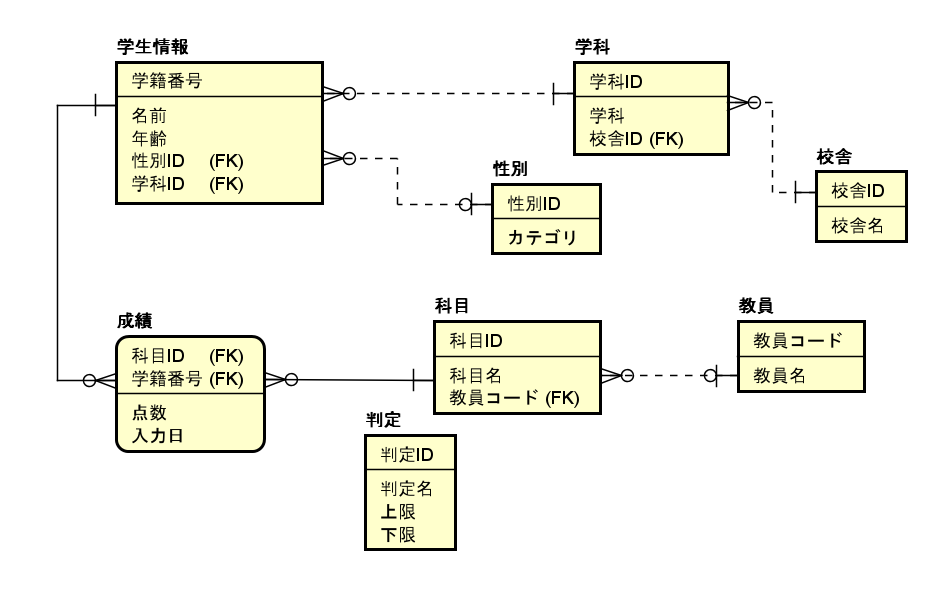
\includegraphics[scale=0.8]{oneER.png}
      \caption{課題1のER図}
       \label{oneER}
      \end{figure}

    \section{課題2}
    本章では課題2におけるプログラムの説明および実行結果について述べる.
    \subsection{プログラムの説明}
    まず,MySQL上にデータベースを定義し接続する.課題2および課題3では「grade」というデータベースを用いる.
    リスト\ref{create}にデータベース「grade」を定義し接続するプログラムを示す.
    リスト\ref{create}において,1行目のクエリがデータベースgradeを定義するクエリである.2行目はコメントアウトしてあるが
    データベースgradeができているか確認することができる.3行目のクエリはデータベースgradeに接続するクエリである.
    \begin{lstlisting}[basicstyle=\ttfamily\footnotesize, frame=single,label=create,caption=データベースの定義および接続]
CREATE DATABASE grade;
-- SHOW DATABASES;
USE grade;
    \end{lstlisting}

    次にテーブルを定義する.テーブルを定義するクエリは,astahでER図(図\ref{oneER})を作成すると自動生成される.
    このため,テーブル定義を行うクエリ全体を説明することは省略する.ここでは学生テーブルの定義クエリを見て,
    どのような命令でテーブル定義を行っているか説明する.リスト\ref{createstudent}に学生テーブルの定義クエリを示す.
    リスト\ref{createstudent}では「CREATE TABLE テーブル名(物理名)」という命令を用いてテーブルを定義していることが読み取れる.
    内部では各カラムについて,「カラム名,型,条件」というようにカラム定義を行っていることが読み取れる.また8,9行目では外部キーの
    設定を行っていることが読み取れる.他のテーブルについても「CREATE TABLE」命令を用いてテーブル定義を行っている.

    \begin{lstlisting}[basicstyle=\ttfamily\footnotesize, frame=single,label=createstudent,caption=学生テーブルの定義]
CREATE TABLE student (
 code CHAR(5) NOT NULL PRIMARY KEY,
 name VARCHAR(40) NOT NULL,
 age INT,
 gender_id INT,
 faculty_id INT NOT NULL,

 FOREIGN KEY (gender_id) REFERENCES gender (gender_id),
 FOREIGN KEY (faculty_id) REFERENCES faculty (faculty_id)
);
    \end{lstlisting}

    テーブル定義ができたから,テーブルにレコードを格納する.レコード格納を行うクエリ全体は非常に長いため,ここでも学生テーブルを例として
    説明する.リスト\ref{recordstudent}に学生テーブルにレコード格納を行うクエリを示す.
    リスト\ref{recordstudent}では「INSERT INTO テーブル名(カラム) VALUES」という命令を用いて
    テーブルにレコードを格納している.他のテーブルについても同様にINSERT命令を用いてレコードを格納している.
 \begin{lstlisting}[basicstyle=\ttfamily\footnotesize, frame=single,label=recordstudent,caption=学生テーブルのレコード格納]
INSERT INTO student(code,name,age,gender_id,faculty_id) VALUES
("26401","山川一郎",18,1,4),
("26205","谷泉太郎",19,1,2),
("26132","海土花子",20,2,1);
\end{lstlisting}

  最後にテーブルの定義およびレコード格納が成功しているか確認する.リスト\ref{test1}に
  全テーブルからレコードを取得するクエリを示す.レコードを取得する命令はSELECTである.
  全レコードを取得する場合は「SELECT * FROM テーブル名」というクエリを発行すると
  テーブル内の全レコードを取得できる.
  \begin{lstlisting}[basicstyle=\ttfamily\footnotesize, frame=single,label=test1,caption=全テーブルからレコードを取得するクエリ]
SELECT * FROM faculty;
SELECT * FROM gender;
SELECT * FROM place;
SELECT * FROM result;
SELECT * FROM score;
SELECT * FROM student;
SELECT * FROM subject;
SELECT * FROM teacher;
  \end{lstlisting}
    \subsection{実行結果}
    実行結果としてリスト\ref{test1}の実行結果を示す.しかし,リスト\ref{test1}の実行結果は非常に長いので
    学生テーブルと成績テーブルについて確認する.図\ref{studentphoto}および図\ref{scorephoto}に,
    リスト\ref{test1}の実行結果を示す.図\ref{studentphoto}は学生テーブルを取得したときの実行結果,
    図\ref{scorephoto}は成績テーブルを取得したときの実行結果である.
    表\ref{one3A}と図\ref{studentphoto}が同じであることから学生テーブルは正常にテーブル定義およびレコード格納が行われている
    ことがわかる.同様に表\ref{one3E}と図\ref{scorephoto}が同じであるから成績テーブルも
    正常であることがわかる.

    \begin{figure}[H]
      \centering
      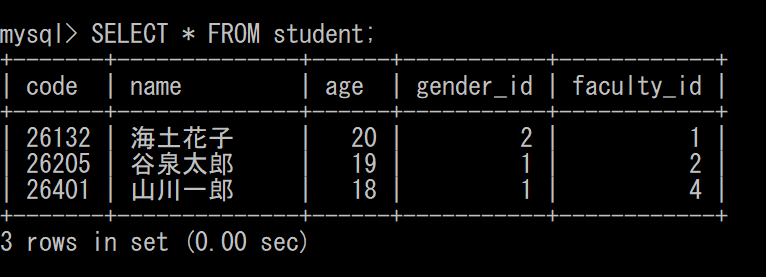
\includegraphics[scale=0.7]{student.png}
      \caption{リスト\ref{test1}の実行結果1}
       \label{studentphoto}
      \end{figure}

      \begin{figure}[H]
        \centering
        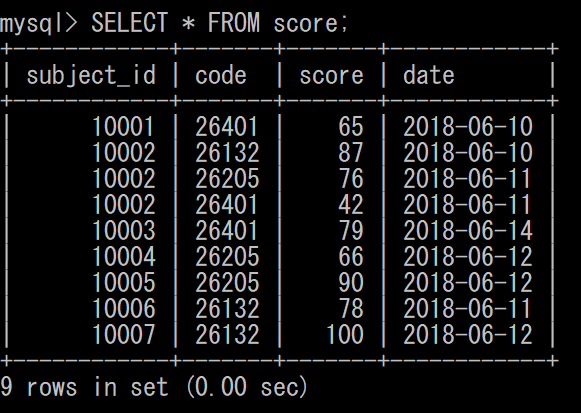
\includegraphics[scale=0.7]{score.png}
        \caption{リスト\ref{test1}の実行結果2}
         \label{scorephoto}
        \end{figure}


    \section{課題3}
    本章では課題3で設けられている5つの課題についてクエリの説明および実行結果について述べる.
    \subsection{クエリの説明}
    本節では問題1~5のクエリについて述べる.
    \subsubsection{問題1のクエリ}
    問題1は第一正規化したときの表を取得するクエリを発行することである.
    問題を言い換えると,MySQLの命令を用いて表\ref{one1}の出力をするクエリを作成することである.
    リスト\ref{q1}に第一正規化した表を取得するクエリを示す.リスト\ref{q1}のクエリでは
    SELECT文を用いてstudent.codeを代表とする必要な項目を出力するように設定する.また,内部結合(INNER JOIN)
    を用いて必要なテーブルを学生テーブルに結合する.内部結合文は「INNER JOIN 結合するテーブル ON 条件」になっている.
    例えば,リスト\ref{q1}の4行目では成績テーブルを成績テーブルの学籍番号と学生テーブルの学籍番号が一致するように
    結合する.また11行目のORDER文は表示結果をソートする命令である.「ORDER BY カラム DESCまたはASC」というように記述する.
    ASCは昇順,DESCは降順のことである.今回は,表\ref{one1}に合わせて,結果を学生の年齢で昇順にソートしている.

    \begin{lstlisting}[basicstyle=\ttfamily\footnotesize, frame=single,label=q1,caption=問題1のクエリ]
 SELECT student.code,student.name,student.age,gender.gender,faculty.faculty,place.place,
 subject.name,score.score,result.result,teacher.teacher_id,teacher.name,score.date
 FROM student  
 INNER JOIN score ON score.code = student.code
 INNER JOIN gender ON student.gender_id = gender.gender_id 
 INNER JOIN faculty ON student.faculty_id = faculty.faculty_id
 INNER JOIN place ON faculty.place_id = place.place_id
 INNER JOIN subject ON subject.subject_id = score.subject_id
 INNER JOIN teacher ON teacher.teacher_id = subject.teacher_id
 INNER JOIN result ON score.score <= result.max AND score.score >= result.min  
 ORDER BY student.age ASC
 ;
        \end{lstlisting}


    \subsubsection{問題2のクエリ}
    問題2は,いずれかの科目の判定が「優」である学生の学籍番号,氏名,学科を問い合わせるクエリを発行し,実行することである.
    リスト\ref{q2}に問題2のクエリを示す.リスト\ref{q2}ではSELECT文と内部結合を用いて必要なテーブルを結合したのちに,
    WHERE文で条件にあったレコードのみを取得する.WHERE文は「WHERE 条件」という文法で用いる.
    ここでは成績テーブルの成績が「優」のレコードのみを取得している.また「DISTINCT」とは取得結果において,
    重複するレコードを重複がなくなるようにする命令のことである
    \begin{lstlisting}[basicstyle=\ttfamily\footnotesize, frame=single,label=q2,caption=問題2のクエリ]
 SELECT DISTINCT student.code,student.name,faculty.faculty
 FROM student INNER JOIN faculty ON faculty.faculty_id = student.faculty_id 
 INNER JOIN score ON score.code = student.code
 INNER JOIN result ON score.score <= result.max AND score.score >= result.min
 WHERE result.result = "優"
 ;
    \end{lstlisting}


    \subsubsection{問題3のクエリ}
問題3は,担当者が「高田」,または「三浦」である科目を履修している学生について,学生名,科目名,点数を問い合わせるクエリを発行し,実行することである.
リスト\ref{q3}に問題3のクエリを示す.リスト\ref{q3}ではSELECT文と内部結合を用いて必要なテーブルを結合したのちに,
WHERE文を用いて条件にあったレコードを取得する.しかしWHERE文の条件が課題2に比べて複雑になっている.
WHERE文の条件がどのようになっているか説明する.まず条件は大きく分けて「OR」という演算子の前と後に分けられる.
前半部分では「teacher.name LIKE 三浦\%」という条件になっている.これはLIKE句を用いて担当教師の名前
が条件にあう文字列のときにTRUEになる.LIKE句は文字列の検索を行う命令で,「LIKE 検索文字列」という文法である.
検索文字列はワイルドカードを使用して,部分検索を行うことができる.今考えている条件は「三浦\%」である.
これは「三浦」の後に0文字以上の任意の文字列を含む文字列という意味である.これによって,担当者が「三浦○○」である
科目のレコードを取得している.命令の後半部分も同様で,担当者が「高田○○」である科目のレコードを取得する.
この2つの命令がOR(論理和)になっているから,問題の「担当者が「高田」,または「三浦」である科目」を取得する
ことができる.

\begin{lstlisting}[basicstyle=\ttfamily\footnotesize, frame=single,label=q3,caption=問題3のクエリ]
 SELECT student.name,subject.name,teacher.name,result.result
 FROM student INNER JOIN score ON score.code = student.code
 INNER JOIN subject ON subject.subject_id = score.subject_id 
 INNER JOIN teacher ON teacher.teacher_id = subject.teacher_id
 INNER JOIN result ON score.score <= result.max AND score.score >= result.min
 WHERE teacher.name LIKE "三浦%" OR teacher.name LIKE "高田%" 
 ORDER BY student.age ASC
 ;
     \end{lstlisting}

    \subsubsection{問題4のクエリ}
    問題4は,科目名に「学」が含まれる科目について,履修している学生名,科目名,点数を問い合わせるクエリを発行し,実行することであった.
    リスト\ref{q4}に問題4のクエリを示す.リスト\ref{q4}ではSELECT文と内部結合を用いて必要なテーブルを結合したのちに,
    WHERE文を用いて条件にあったレコードを取得する.WHERE文の条件は,科目テーブルの科目名がLIKE句以下の条件に当てはまるときである.
    LIKE句の条件は「\%学\%」である.\%は課題3のクエリで説明したように0文字以上の任意の文字列である.
    「\%学\%」にすることで「統計学」のように一番後ろの文字が「学」である場合も「力学I」のように途中に「学」が
    入っている場合も検出できる.
    \begin{lstlisting}[basicstyle=\ttfamily\footnotesize, frame=single,label=q4,caption=問題4のクエリ]
 SELECT student.name,subject.name,score.score
 FROM student INNER JOIN score ON score.code = student.code
 INNER JOIN subject ON subject.subject_id = score.subject_id 
 WHERE subject.name LIKE "%学%"
 ORDER BY student.age ASC
 ;
          \end{lstlisting}

    \subsubsection{問題5のクエリ}
    問題5は担当が「三浦」の科目の平均点を問い合わせるクエリを発行し,実行することである.
    リスト\ref{q5}に問題5のクエリを示す.リスト\ref{q5}ではSELECT文で「AVG(score.score)」を
    画面出力する.AVGとはaverage(平均)のことである.ここでの平均は算術平均をことである.
    リスト\ref{q5}では科目の平均点を問い合わせるので成績テーブルの成績の平均を出力している.
    また,WHERE文の条件としては問題3のクエリ(リスト\ref{q3})を流用している.
        \begin{lstlisting}[basicstyle=\ttfamily\footnotesize, frame=single,label=q5,caption=問題5のクエリ]
 SELECT AVG(score.score)
 FROM student INNER JOIN score ON score.code = student.code
 INNER JOIN subject ON subject.subject_id = score.subject_id 
 INNER JOIN teacher ON teacher.teacher_id = subject.teacher_id
 WHERE teacher.name LIKE "三浦%"
 ;
          \end{lstlisting}


    \subsection{実行結果}
    本節では問題1~問題5のクエリの実行結果について述べる.
    \subsubsection{問題1の実行結果}
    課題1のクエリ(リスト\ref{q1})の実行結果の図は横に長いため,掲載を省略する.
    実行結果は表\ref{one1}の第一正規化の結果と一致していることが確認できた.
    これよりリスト\ref{q1}のクエリは課題1の題意は満たせたと言える.

    \subsubsection{問題2の実行結果}
    課題2のクエリ(リスト\ref{q2})の実行結果を図\ref{kadai3-2}に示す.
    表\ref{one1}から,判定に「優」がある学生は「谷川太郎」と「海土花子」であることが
    わかる.すなわち,問題2のクエリの正しい実行結果として,この2人の学籍番号,氏名,学科が取得できればよい.
    図\ref{kadai3-2}を見ると,この2人の学籍番号,氏名,学科が取得できていることがわかる.
    これよりリスト\ref{q2}のクエリは課題2の題意は満たせたと言える.

    \begin{figure}[H]
      \centering
      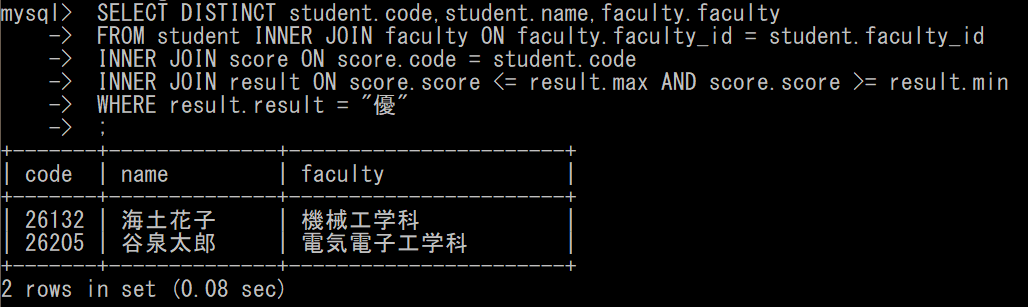
\includegraphics[scale=0.9]{kadai3-2.png}
      \caption{リスト\ref{q2}の実行結果}
       \label{kadai3-2}
      \end{figure}

    \subsubsection{問題3の実行結果}
    課題3のクエリ(リスト\ref{q3})の実行結果を図\ref{kadai3-3}に示す.
    表\ref{one1}から,担当者が「高田」,または「三浦」である科目を履修している学生とその科目は
    「山川一郎」が「現代社会」,「谷川太郎」が「信号処理」,「電気工学」であることがわかる.
    すなわち,課題3のクエリの正しい実行結果として,この3つの科目において,履修学生の氏名,科目名,点数が取得できればよい.
    またここでは確認のために担当者の名前も表示する.図\ref{kadai3-2}を見ると,この3つの科目の履修学生の氏名,科目名,点数
    が取得できていることがわかる.これよりリスト\ref{q3}のクエリは課題3の題意は満たせたと言える.

    \begin{figure}[H]
      \centering
      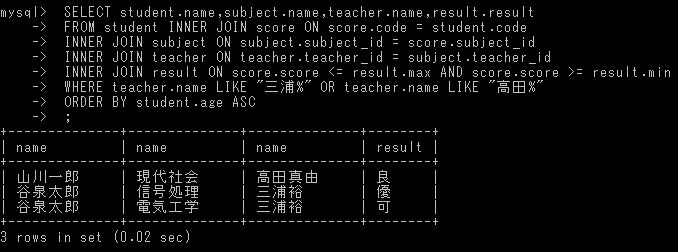
\includegraphics[scale=1.2]{kadai3-3.png}
      \caption{リスト\ref{q3}の実行結果}
       \label{kadai3-3}
      \end{figure}

    \subsubsection{問題4の実行結果}
    課題4のクエリ(リスト\ref{q4})の実行結果を図\ref{kadai3-4}に示す.
    表\ref{one1}から,「学」が含まれる科目は「電気工学」,「機械工学」,「計測工学」の3つ
    であることがわかる.すなわち,課題4のクエリの正しい実行結果として,この3つの科目を履修している学生名,科目名,点数
    が取得できればよい.図\ref{kadai3-4}を見ると,この3つの科目を履修している科目の学生名,科目名,点数が取得できている
    ことがわかる.これよりリスト\ref{q4}のクエリは課題4の題意は満たせたと言える.

    \begin{figure}[H]
      \centering
      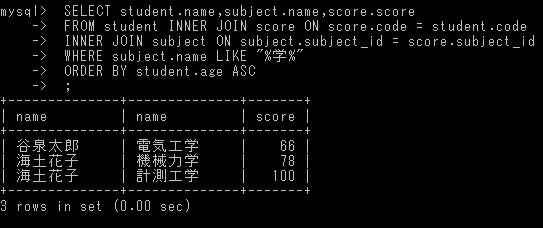
\includegraphics[scale=1.2]{kadai3-4.png}
      \caption{リスト\ref{q4}の実行結果}
       \label{kadai3-4}
      \end{figure}

    \subsubsection{問題5の実行結果}
    課題5のクエリ(リスト\ref{q5})の実行結果を図\ref{kadai3-5}に示す.
    表\ref{one1}から,担当者が「三浦」である科目は2つあり,それぞれ66点と99点であることがわかる.
    すなわち平均点は78点である.これが実行結果として取得できればよい.
    図\ref{kadai3-5}を見ると,平均点として78.0点が取得できていることがわかる.
    これよりリスト\ref{q5}のクエリは課題5の題意は満たせたと言える.

    \begin{figure}[H]
      \centering
      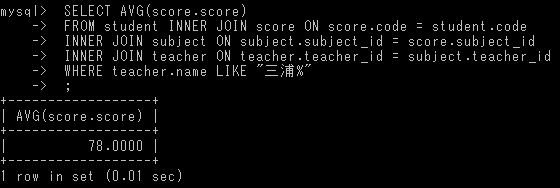
\includegraphics[scale=1.2]{kadai3-5.png}
      \caption{リスト\ref{q5}の実行結果}
       \label{kadai3-5}
      \end{figure}

    \section{課題4}
    本章では課題4として次に示す項目について述べる.
    \begin{enumerate}
      \item データの概要および目的
      \item データの正規化とER図
      \item MySQLによる実装
      \item 実装結果
      \item テスト項目
      \item テスト項目のプログラムの説明
      \item テスト項目の実行結果
    \end{enumerate}

    \subsection{データの概要および目的}
    課題4として長野市のオープンデータである「避難場所の一覧」を用いる\cite{open}.このオープンデータを用いる目的として,
    近年の自然災害の多さから,避難場所を検索するデータベースを作成し,付近の避難場所を検索を行うことを
    目的とする.オープンデータ「避難場所の一覧」は2020年8月4日現在,2020年4月7日に最終更新されたデータである.\\
    レコード数は202でカラムの一覧は次に示す通りである.ここで適否とは避難に適しているか否かの情報であるから
    ○もしくは×のどちらかである.また指定避難所,広域避難場所は指定されている場合○,それ以外の場合はハイフンまたは
    空欄になっている.洪水,土砂災害,地震は留意事項の項目があるが,大規模な火事には留意事項がないことも注意が必要である.
    \begin{enumerate}
      \item ID
      \item 指定緊急避難場所の名称(以下,避難場所名)
      \item 名称かな
      \item 住所
      \item 所在地区
      \item 緯度
      \item 経度
      \item 洪水等の適否
      \item 洪水等の適否(留意事項)
      \item 土砂災害の適否
      \item 土砂災害の適否(留意事項)
      \item 地震の適否
      \item 地震の適否(留意事項)
      \item 大規模な火事の適否
      \item 指定避難所
      \item 広域避難場所
    \end{enumerate}

    \subsection{データの正規化とER図}
    データの正規化を行う.元のデータはカラム数が多いため掲載は省略する.また,元のデータは
    レコードをまたいで定義される値がない.このため第一正規化はすでに完了しているのと同義である.\\
     第二正規化を行う.ここでは3つのテーブルに分離する.1つ目はIDを主として,避難場所名,名称かな,住所,所在地区,緯度,経度
    の6カラムを従属するカラムとする(避難場所テーブル).2つ目はIDを主として,洪水,土砂災害,地震,大規模な火事の適否とその留意事項の合計7カラムを
    従属するカラムとする(避難適否テーブル).3つ目はIDを主として指定避難所,広域避難場所を従属するカラムとする(避難場所属性テーブル).これらを表で表すと表\ref{four21}~表\ref{four23}
    のようになる.表\ref{four21}~表\ref{four23}では各カラムについて最初の3行を表示している.ただし,避難場所テーブル(表\ref{four21})の「名称かな」は長いため
    省略する.
    \begin{table}[H]
      \caption{避難場所テーブル}
      \label{four21}
      \begin{center}
        \scalebox{0.7}[0.9]{
          \begin{tabular}{c|c|c|c|c|c|c}\hline
            ID & 避難場所名 & 名称かな & 住所 & 所在地区 & 緯度 & 経度 \\ \hline \hline
            1 & 長野市立加茂小学校 & (省略) & 長野県長野市大字西長野185-6 & 01第一 & 36.65751141 & 138.1764597 \\ \hline
            2 & 信州大学教育学部グラウンド & (省略) & 長野県長野市西長野6の口 & 01第一 & 36.65736035 & 138.1798011 \\ \hline
            3 & ひまわり公園 & (省略) & 長野県長野市大字長野旭町1108-10 & 01第一 & 36.65470572 & 138.1824138 \\ \hline
            $\vdots$ & $\vdots$ & $\vdots$ & $\vdots$ & $\vdots$ & $\vdots$ & $\vdots$\\ \hline
          \end{tabular}
        }
      \end{center}
      \end{table}

      \begin{table}[H]
        \caption{避難適否テーブル}
        \label{four22}
        \begin{center}
          \scalebox{0.7}[0.9]{
            \begin{tabular}{l|c|c|c|c|c|c}\hline
              ID & 洪水等の適否 & 洪水等の適否(留意事項) & 土砂災害の適否 & 土砂災害の適否(留意事項) & 地震の適否  & 大規模な火事の適否 \\ \hline \hline
              1 & ○ & グラウンド除く & ○ &  & ○ & × \\ \hline
              2 & ○ &  & ○ & 北西の一部除く & ○ & × \\ \hline
              3 & ○ &  & ○ &  & ○ & × \\ \hline
              $\vdots$ & $\vdots$ & $\vdots$ & $\vdots$ & $\vdots$ & $\vdots$ & $\vdots$\\ \hline
            \end{tabular}
          }
        \end{center}
        \end{table}

        \begin{table}[H]
          \caption{避難場所属性テーブル}
          \label{four23}
          \begin{center}
              \begin{tabular}{c|c|c}\hline
                ID & 指定避難所 & 広域避難場所 \\ \hline
                1 & ○ & \\ \hline
                2 & - & \\ \hline
                3 & - & \\ \hline
                $\vdots$ & $\vdots$ & $\vdots$ \\ \hline
              \end{tabular}
          \end{center}
          \end{table}
        
          次に第三正規化を行う.避難場所テーブル(表\ref{four21})において所在地区は一定の選択肢から
          選ぶ項目になっているため,分離する.また,避難適否テーブル(表\ref{four22})において留意事項
          も一定の選択肢から選ぶか,空欄となっているから分離する.避難場所属性テーブル(表\ref{four23})
          は○,-,空白の扱いが入り乱れているため,○もしくは×に統一する.表\ref{four31}~表\ref{four35}に第三正規化
          したテーブルを示す.土砂災害,地震,火災の適否テーブルおよび留意事項テーブルは洪水テーブルと同様のものであるから
          省略する.

          \begin{table}[H]
            \caption{避難場所テーブル}
            \label{four31}
            \begin{center}
              \scalebox{0.7}[0.9]{
                \begin{tabular}{c|c|c|c|c|c|c}\hline
                  ID & 避難場所名 & 名称かな & 住所 & 所在地区 & 緯度 & 経度 \\ \hline \hline
                  1 & 長野市立加茂小学校 & (省略) & 長野県長野市大字西長野185-6 & 1 & 36.65751141 & 138.1764597 \\ \hline
                  2 & 信州大学教育学部グラウンド & (省略) & 長野県長野市西長野6の口 & 1 & 36.65736035 & 138.1798011 \\ \hline
                  3 & ひまわり公園 & (省略) & 長野県長野市大字長野旭町1108-10 & 1 & 36.65470572 & 138.1824138 \\ \hline
                  $\vdots$ & $\vdots$ & $\vdots$ & $\vdots$ & $\vdots$ & $\vdots$ & $\vdots$\\ \hline
                \end{tabular}
              }
            \end{center}
            \end{table}

            \begin{table}[H]
              \begin{center}
                \begin{tabular}{c}

                  \begin{minipage}{0.5\hsize}
            \caption{所在地区テーブル}
            \label{four32}
            \begin{center}
                \begin{tabular}{c|c}\hline
                  所在地区ID & 所在地区名 \\ \hline \hline
                  1 & 01第一 \\ \hline
                  2 & 02第二 \\ \hline 
                  3 & 03第三 \\ \hline
                  $\vdots$ & $\vdots$ \\ \hline
                  4 & 44大岡 \\ \hline
                  5 & 45信州新町 \\ \hline
                  6 & 46中条 \\ \hline                  
                \end{tabular}
            \end{center}
          \end{minipage}

          \begin{minipage}{0.5\hsize}
              \caption{避難場所の属性テーブル}
              \label{four33}
              \begin{center}
                  \begin{tabular}{c|c|c}\hline
                    ID & 指定避難所 & 広域避難場所 \\ \hline \hline
                    1 & ○ & × \\ \hline
                    2 & × & × \\ \hline
                    3 & × & × \\ \hline
                    $\vdots$ & $\vdots$ & $\vdots$ \\ \hline
                  \end{tabular}
              \end{center}
            \end{minipage}
          \end{tabular}
        \end{center}
              \end{table}

              \begin{table}[H]
                \begin{center}
                  \begin{tabular}{c}
  
                    \begin{minipage}{0.5\hsize}
              \caption{洪水テーブル}
              \label{four34}
              \begin{center}
                  \begin{tabular}{c|c|c}\hline
                    ID & 避難の適否 & 留意事項 \\ \hline \hline
                    1 & ○ & 1 \\ \hline
                    2 &	○ &	0 \\ \hline
                    3 &	○ &	0 \\ \hline
                    $\vdots$ & $\vdots$ & $\vdots$ \\ \hline
                  \end{tabular}
              \end{center}
            \end{minipage}
  
            \begin{minipage}{0.5\hsize}
                \caption{洪水留意事項テーブル}
                \label{four35}
                \begin{center}
                    \begin{tabular}{c|l}\hline
                      留意事項ID & 留意事項 \\ \hline \hline
                      0 & なし \\ \hline 
                      1 & グラウンド除く \\ \hline
                      2 & 体育館除く \\ \hline
                      3 & 2階以上 \\ \hline
                      4 & \begin{tabular}{c} 2階部分の観客席及び \\ 内部・外部コンコース \end{tabular} \\ \hline
                    \end{tabular}
                \end{center}
              \end{minipage}
            \end{tabular}
          \end{center}
                \end{table}

    第三正規化ができたから,ER図の作成を行う.図\ref{kadai4ER}にER図を示す.
    \begin{figure}[H]
      \centering
      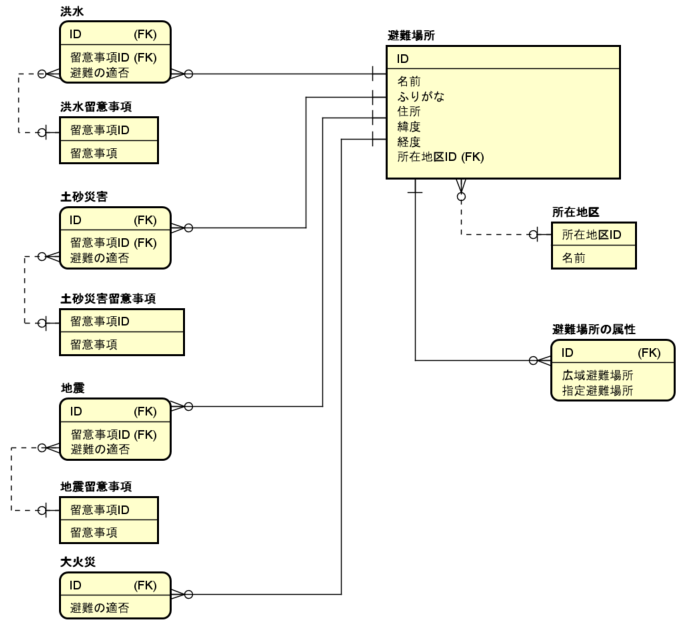
\includegraphics[scale=1.0]{kadai4ER.png}
      \caption{課題4のER図}
       \label{kadai4ER}
      \end{figure}

    \subsection{MySQLによる実装}
    MySQLで避難場所データベースを実装する.表\ref{joken4}にカラムの設定を示す.
     \begin{table}[H]
      \caption{カラムの設定}
      \label{joken4}
      \begin{center}
        \begin{tabular}{l|l|l|l|l}\hline
          項目 & カラム(論理名) & カラム(物理名) & 型 & 必須/非必須 \\ \hline \hline
          ID & ID & code & INT & 必須 \\ \hline
          避難所名 & 名前 & name & VARCHAR(100) & 必須 \\ \hline
          名称かな & ふりがな & kana & VARCHAR(100) & 必須 \\ \hline
          住所 & 住所 & address & VARCHAR(50) & 必須 \\ \hline
          緯度 & 緯度 & latitude & FLOAT(10) & 必須 \\ \hline
          経度 & 経度 & longitude & FLOAT(10) & 必須 \\ \hline
          所在地区ID & 所在地区ID & district\_id & INT & 必須 \\ \hline
          所在地区 & 所在地区名 & name & VARCHAR(10) & 必須 \\ \hline
          広域避難場所 & 広域避難場所 & wide\_area & CHAR(2) & 非必須 \\ \hline
          指定避難所 & 指定避難所 & designation & CHAR(2) & 非必須 \\ \hline
          避難の適否 &  避難の適否 & suitability & CHAR(2) & 必須 \\ \hline
          留意事項 & 留意事項 & note & VARCHAR(50) & 非必須 \\ \hline
        \end{tabular}
      \end{center}
      \end{table}

      避難場所データベースをデータベース名を「evacuation」として定義する.また,表\ref{joken4}に示す条件で,避難場所データベースのテ
      ーブル定義クエリをastahで生成し定義する.さらに,テーブルにレコードを追加するクエリを発行して,実行する.
      データベース定義クエリおよびレコード追加クエリは非常に長いため省略する.
    \subsection{実装結果}
    テーブルが正しく生成できているか確認する.ここでは,SELECT文を用いて避難場所テーブルおよび洪水テーブルが正しく生成できているか確認する.
      リスト\ref{check}避難場所テーブルおよび洪水テーブルの全レコードを取得するクエリを示す.
      \begin{lstlisting}[basicstyle=\ttfamily\footnotesize, frame=single,label=check,caption=実装結果を確認するためのクエリ]
 SELECT * FROM place;
 SELECT * FROM flood;
                 \end{lstlisting}
    避難場所テーブルの場合の実行結果は非常に長いため省略するが,全レコードを問題なく取得できた.
    図\ref{flood}に洪水テーブルにおける実行結果の抜粋を示す.図\ref{flood}は表\ref{four34}と同じであるから
    正しく実装できていると言える.
    \begin{figure}[H]
      \centering
      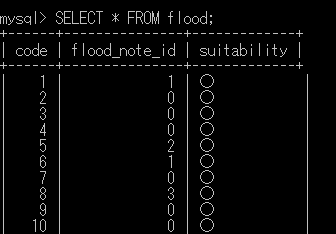
\includegraphics[scale=1.0]{flood.png}
      \caption{洪水レコードの実装の確認}
       \label{flood}
      \end{figure}


    \subsection{テスト項目}
    課題3と同様に次の5つのクエリを発行し,実行する.
    \begin{enumerate}
      \item 第一正規化したときの表を取得するクエリ.
      \item 広域避難場所に指定されている避難場所の番号,名前,所在地区を問い合わせるクエリ.
      \item 所在地区が「朝陽」,「豊野」の避難場所の名前,所在地区,各災害の避難の適否を問い合わせるクエリ.
      \item 避難場所の名前に「学校」が含まれている避難場所について避難場所の名前,所在地区,避難所の属性を問い合わせるクエリ.
      \item 現在地(緯度,経度)から最も近い避難場所の名前,住所,緯度,経度を問い合わせるクエリ.
    \end{enumerate}    
    \subsection{クエリの説明}
    本節では問題1~5のクエリについて述べる.
    \subsubsection{問題1のクエリ}
    問題1は第一正規化したときの表を取得するクエリを発行し,実行することであった.
    リスト\ref{qq1}に問題1のクエリを示す.リスト\ref{qq1}ではすべてのテーブルを内部結合し,SELECT文を用いて表示
    している.
    \begin{lstlisting}[basicstyle=\ttfamily\footnotesize, frame=single,label=qq1,caption=問題1のクエリ]
SELECT place.code,place.name,place.kana,place.address,
place.latitude,place.longitude,district.name,
attribute.designation,attribute.wide_area,
flood.suitability,flood_note.note,
sediment_disaster.suitability,sediment_disaster_note.note,
earthquake.suitability,earthquake_note.note,
fire.suitability
FROM place
INNER JOIN district ON district.district_id = place.district_id
INNER JOIN attribute ON attribute.code = place.code
INNER JOIN flood ON flood.code = place.code
INNER JOIN sediment_disaster ON sediment_disaster.code = place.code
INNER JOIN earthquake ON earthquake.code = place.code
INNER JOIN fire ON fire.code = place.code
INNER JOIN flood_note ON flood_note.flood_note_id = flood.flood_note_id
INNER JOIN sediment_disaster_note ON sediment_disaster_note.sediment_disaster_notes_id 
= sediment_disaster.sediment_disaster_notes_id
INNER JOIN earthquake_note ON earthquake_note.earthquake_note_id 
= earthquake.earthquake_note_id
;
               \end{lstlisting}

    \subsubsection{問題2のクエリ}
    問題2は広域避難場所に指定されている避難場所の番号,名前,所在地区を問い合わせるクエリを発行し,実行することであった.
    リスト\ref{qq2}に問題2のクエリを示す.リスト\ref{qq2}ではSELECT文を用いて必要なテーブルを結合したのち,
    WHERE文を用いて広域避難場所に指定されているレコードのみを取得している.
    \begin{lstlisting}[basicstyle=\ttfamily\footnotesize, frame=single,label=qq2,caption=問題2のクエリ]
SELECT place.code,place.name,district.name
FROM place
INNER JOIN district ON district.district_id = place.district_id
INNER JOIN attribute ON attribute.code = place.code
WHERE attribute.wide_area = "○"
;
    \end{lstlisting}
    \subsubsection{問題3のクエリ}
問題3は所在地区が「朝陽」,「豊野」の避難場所の名前,所在地区,各災害の避難の適否を問い合わせるクエリを発行し,実行することであった.
リスト\ref{qq3}に問題3のクエリを示す.リスト\ref{qq3}えはSELECT文を用いて必要なテーブルを結合したのち,
WHERE文を用いて所在地区が「朝陽」,「豊野」であるレコードを取得している.
\begin{lstlisting}[basicstyle=\ttfamily\footnotesize, frame=single,label=qq3,caption=問題3のクエリ]
SELECT place.name,district.name,flood.suitability,
sediment_disaster.suitability,earthquake.suitability,fire.suitability
FROM place
INNER JOIN district ON district.district_id = place.district_id
INNER JOIN flood ON flood.code = place.code
INNER JOIN sediment_disaster ON sediment_disaster.code = place.code
INNER JOIN earthquake ON earthquake.code = place.code
INNER JOIN fire ON fire.code = place.code
WHERE district.name = "朝陽" OR district.name = "豊野" 
;
      \end{lstlisting}

    \subsubsection{問題4のクエリ}
問題4は避難場所の名前に「学校」が含まれている避難場所について避難場所の名前,所在地区,避難所の属性を問い合わせるクエリを発行し,実行することであった.
リスト\ref{qq4}に問題4のクエリを示す.リスト\ref{qq4}ではSELECT文を用いて必要なテーブルを結合したのち,WHERE文とLIKE句を
用いて「学校」を含むレコードを取得している.
\begin{lstlisting}[basicstyle=\ttfamily\footnotesize, frame=single,label=qq4,caption=問題4のクエリ]
SELECT place.name,district.name,attribute.designation,attribute.wide_area
FROM place
INNER JOIN district ON district.district_id = place.district_id
INNER JOIN attribute ON attribute.code = place.code
WHERE place.name LIKE "%学校%"
;
\end{lstlisting}

    \subsubsection{問題5のクエリ}
    問題5は現在地(緯度経度)から最も近い避難場所の名前,住所,緯度,経度を問い合わせるクエリを発行し,実行することであった.
    リスト\ref{qq5}に問題5のクエリを示す.リスト\ref{qq5}ではSELECT文を用いて,必要なテーブルを結合したのちに,
    緯度,経度の情報から,避難場所までの距離を計算し,近くにある避難場所を取得する.
    点P(緯度,経度)と表すことにすると,2点A($x_1,y_2$),B($x_1,y_2$)の距離$d$は式(\ref{idokeido})で
    表される\cite{idokeido}.ただし,赤道半径$r = 6378 km$とする.距離の計算結果をLIMIT文を用いて距離が近い順に,上位5件
    取得する.
    \begin{lstlisting}[basicstyle=\ttfamily\footnotesize, frame=single,label=qq5,caption=問題5のクエリ]
SELECT place.name,place.address,place.latitude,place.longitude,( 
    6371 * ACOS( 
      COS(RADIANS(現在地(緯度))) * COS(RADIANS(place.LATITUDE)) * 
      COS(RADIANS(place.LONGITUDE) - RADIANS(現在地(経度)))
       + SIN(RADIANS(現在地(緯度))) * SIN(RADIANS(place.LATITUDE))
    )
  ) AS DISTANCE 
FROM place
ORDER BY DISTANCE 
LIMIT 5
;
      \end{lstlisting}

      \begin{equation}
        d = r \cos^{-1}\left( \cos y_1 \cos y_2 \cos(x_2 - x_1) + \sin y_1 \sin y_2  \right)
        \label{idokeido}
      \end{equation}
    \subsection{実行結果}
    本節では問題1~5の実行結果について述べる.
    \subsubsection{問題1の実行結果}
    問題1の実行結果は非常に長いため省略するが,第一正規化の表を取得することができた.
    これより問題1の題意は満たせたと言える.
    \subsubsection{問題2の実行結果}
    図\ref{kadai4-2}に問題2のクエリ(リスト\ref{qq2})の実行結果を示す.
    長野市の広域避難場所は長野市のホームページの「避難場所・避難所・福祉避難所・応急救護所・防災備蓄倉庫について」\cite{hinan}より
    図\ref{kadai4-2}の実行結果で取得した5件であることがわかる.これより,問題2の題意を満たせたと言える.

    \begin{figure}[H]
      \centering
      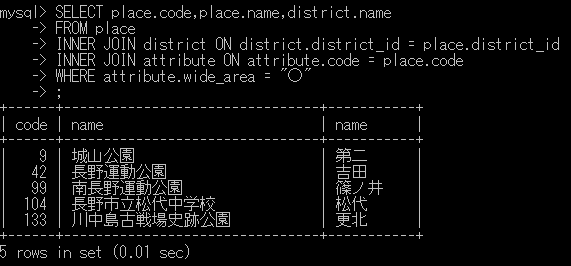
\includegraphics[scale=1.0]{kadai4-2.png}
      \caption{問題2の実行結果}
       \label{kadai4-2}
      \end{figure}

    \subsubsection{問題3の実行結果}
    図\ref{kadai4-3}に問題3のクエリ(リスト\ref{qq3})の実行結果を示す.
    第一正規化したデータと図\ref{kadai4-3}の実行結果を比較すると,所在地区が「朝陽」,「豊野」
    のレコードを正しく取得できていると言える.これより問題3の題意は満たせたと言える.

    \begin{figure}[H]
      \centering
      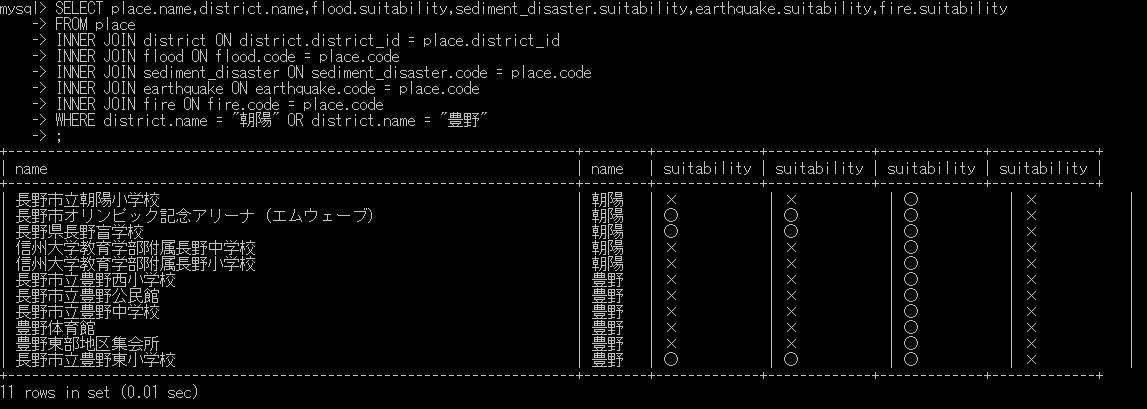
\includegraphics[scale=0.7]{kadai4-3.png}
      \caption{問題3の実行結果}
       \label{kadai4-3}
      \end{figure}

    \subsubsection{問題4の実行結果}
    図\ref{kadai4-4}に問題4のクエリ(リスト\ref{qq4})の実行結果の冒頭を示す.
    図\ref{kadai4-4}から,避難場所名に「学校」を含むレコードを取得できていることがわかる.
    これより,課題4の題意は満たせたと言える.

    \begin{figure}[H]
      \centering
      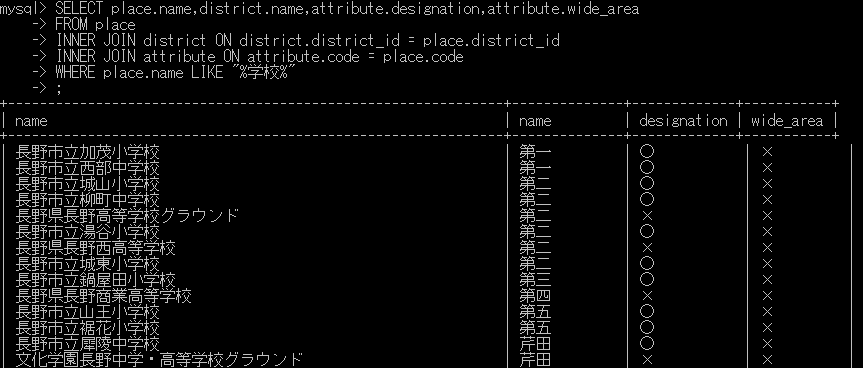
\includegraphics[scale=1.0]{kadai4-4.png}
      \caption{問題4の実行結果}
       \label{kadai4-4}
      \end{figure}

    \subsubsection{問題5の実行結果}
    図\ref{kadai4-5-1}および図\ref{kadai4-5-2}に問題4のクエリ(リスト\ref{qq5})の実行結果を示す.
    図\ref{kadai4-5-1}は長野高専の緯度,経度の場合の実行結果,図\ref{kadai4-5-2}は長野駅の緯度,経度
    の場合の実行結果である.長野高専の場合,長野高専のグラウンド,市立長野高校,徳間小学校が取得されている.
    これは正しい結果であると言える.また,長野駅の場合,長野駅東口の公園,長野市立鍋屋田小学校が取得されている.
    これも正しい結果であると言える.これらより,課題5の題意は満たせたと言える.

      \begin{figure}[H]
      \centering
      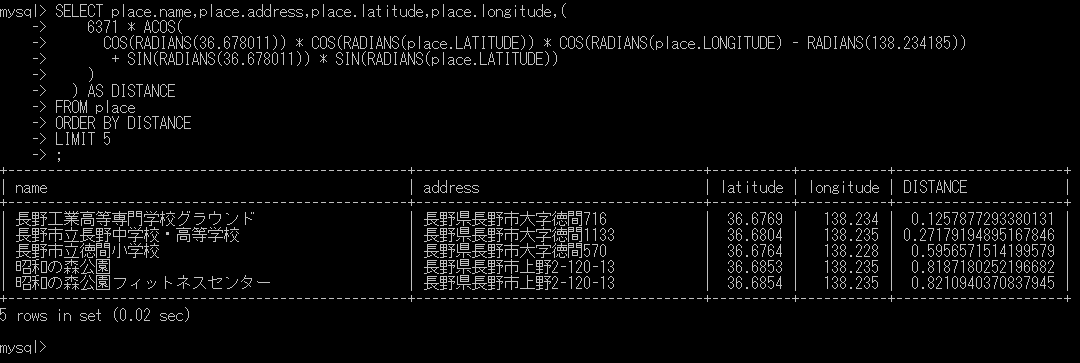
\includegraphics[scale=0.7]{kadai4-5-1.png}
      \caption{問題5の実行結果(座標:長野高専)}
       \label{kadai4-5-1}
      \end{figure}

      \begin{figure}[H]
        \centering
        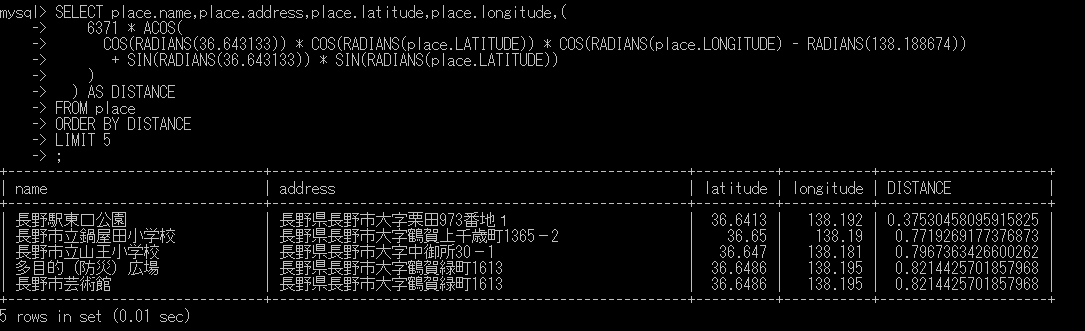
\includegraphics[scale=0.7]{kadai4-5-2.png}
        \caption{問題5の実行結果(座標:長野駅)}
         \label{kadai4-5-2}
        \end{figure}

    \section{考察}
        課題1~3について,簡単なデータで正規化やER図,MySQLでの実装を学習することができた.これより,
        正規化やSQLの使い方について学習するという目的を達成できたと言える.課題4については,
        また,課題4について,長野市のオープンデータを用いてデータベースを作成できた.しかし第二正規化,第三正規化が
        非常に簡素であり,正規化の有効性や拡張性を理解ためのデータとしてはあまりふさわしくないと考える.
        しかし問題5で作成したクエリは任意の座標(緯度,経度)から付近の避難所を検索することができるため,実用性が
        あると考える.このことから長野市のオープンデータを用いて,実際に役に立つデータベースやクエリを作成することができた
        と考える.

        \begin{thebibliography}{9}
          \bibitem{NNCT}  国立高専機構長野高専,\url{http://www.nagano-nct.ac.jp/} ,閲覧日2020年8月5日
          \bibitem{open}  長野市オープンデータサイト,\url{https://www.city.nagano.nagano.jp/site/opendata/} ,閲覧日2020年8月5日
          \bibitem{idokeido} 三浦英俊,"緯度経度を用いた3つの距離計算方法",\url{http://www.orsj.or.jp/archive2/or60-12/or60_12_701.pdf},閲覧日2020年8月5日
          \bibitem{hinan}  避難場所・避難所・福祉避難所・応急救護所・防災備蓄倉庫について,\url{https://www.city.nagano.nagano.jp/soshiki/kikibousai/2530.html} ,閲覧日2020年8月5日
        \end{thebibliography}

\end{document}

